\section{\translate{Results}}\label{sec:results}
Summarize and introduce your results

\subsection{\translate{Resulting application}/\translate{Resulting system}}\label{subsec:resultapp}
Present your resulting work. Screenshots, features, etc.

\subsection{\translate{Measurement results}}\label{subsec:measurementresults}
Present your measurements. How well does it perform? Present the results objectively, with as little
bias as possible. Use tables, graphs, etc.  You can find an example table below. See Table 1.

\begin{table}
  \caption{Measured times for the model.}
  \begin{tabular}{c c c c c}
              & Shortest (ms) & Longest (ms) & Average (ms) & Stdev (ms)\\
    \toprule
    Model one & 10 & 30 & 20 & 5 \\
    \midrule 
    Model two & 20 & 40 & 35 & 3 \\
    \bottomrule
  \end{tabular}
\end{table}

Here is an example of a line graph. See~\cref{fig:line}.
\begin{figure}
  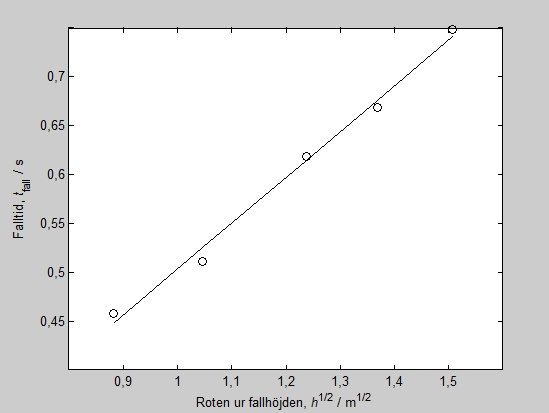
\includegraphics[width=5cm]{Figures/graph1.png}
  \caption{Line graph example.}\label{fig:line}
\end{figure}

Here is an example of a bar chart with standard deviation whiskers. See~\cref{fig:bar}.
\begin{figure}
  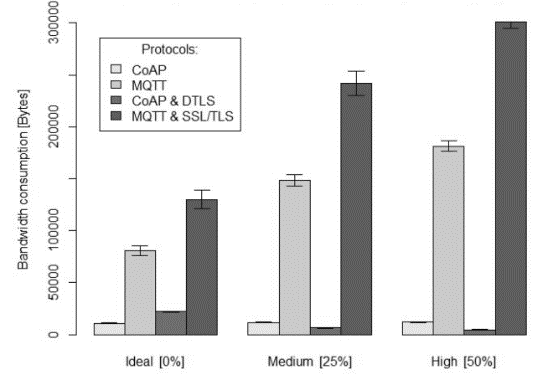
\includegraphics[width=5cm]{Figures/graph2.png}
  \caption{Bar chart example.}\label{fig:line}
\end{figure}

Here is an example boxplot. See~\cref{fig:boxplot}

\begin{figure}
  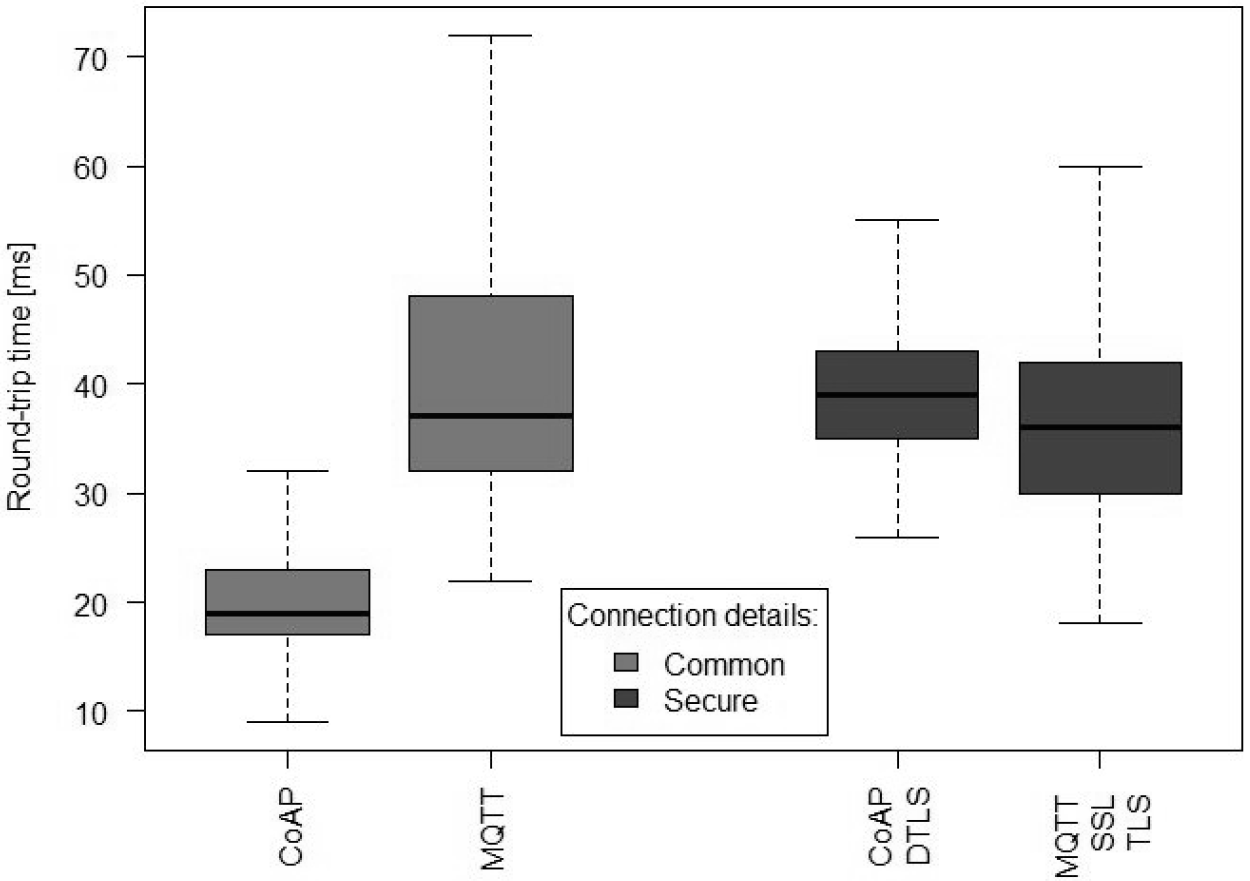
\includegraphics[width=5cm]{Figures/graph3.png}
  \caption{Boxplot example.}\label{fig:line}
\end{figure}

Here is an example equation. See~\cref{eqn:exampleeqn}

\begin{equation}
  P_{i,j} = C\frac{P_iG_{i,j}}{d^a_{i,j}}
\end{equation}
